\documentclass[border=4pt]{standalone}
\usepackage{tikz}
\usetikzlibrary{arrows.meta,positioning,shapes.geometric}
\tikzset{
  block/.style={draw,minimum width=20mm,minimum height=9mm,align=center},
  sensor/.style={circle,draw,minimum size=10mm,inner sep=1pt},
  threshold/.style={diamond,draw,aspect=1.8,inner sep=1pt,align=center}
}
\begin{document}
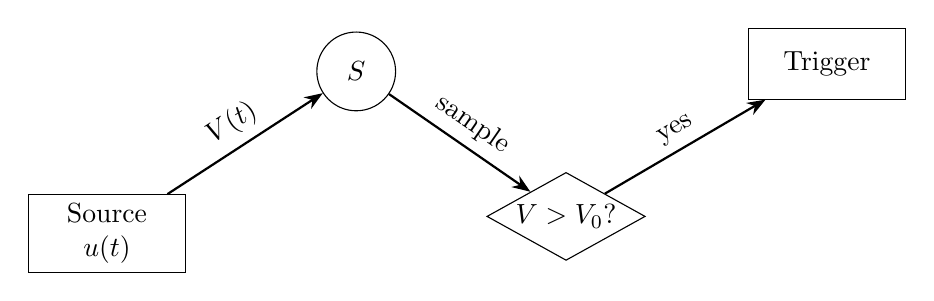
\begin{tikzpicture}[node distance=12mm and 18mm,>=Stealth]
  \node[block] (source) {Source\\$u(t)$};
  \node[sensor,above right=of source] (sensor) {$S$};
  \node[threshold,below right=of sensor] (limit) {$V>V_0?$};
  \node[block,above right=of limit] (trigger) {Trigger};
  \draw[->,thick] (source) -- node[above,sloped] {$V(t)$} (sensor);
  \draw[->,thick] (sensor) -- node[above,sloped] {sample} (limit);
  \draw[->,thick] (limit) -- node[above,sloped] {yes} (trigger);
\end{tikzpicture}
\end{document}
